% !TeX program = lualatex
\documentclass[usenames,dvipsnames]{beamer}
\usepackage{array}
\usepackage{colortbl}
\usetheme{upctelecos}

%%% Some useful commands
% pdf-friendly newline in links
\newcommand{\pdfnewline}{\texorpdfstring{\newline}{ }} 
% Fill the vertical space in a slide (to put text at the bottom)
\newcommand{\framefill}{\vskip0pt plus 1filll}

\title[FAPEC]{Implementation of FAPEC decorrelation stages for IQ and water column data}
\date[July 2021]{Barcelona, July 2021}
\author[Aniol Martí]{
  Author: Aniol Martí\\
  Supervised by: Ferran de Cabrera, Jordi Portell, Jaume Riba
}
\institute{Universitat Politècnica de Catalunya}

\begin{document}
\begin{frame}
\titlepage
\end{frame}

\begin{frame}{Outline}
\tableofcontents
\end{frame}

\AtBeginSection[]
{
\begin{frame}{Outline}
\tableofcontents[currentsection]
\end{frame}
}

\section{Introduction}
\begin{frame}{Background}
\begin{itemize}
	\item Two strategic projects of DAPCOM Data Services, a spin-off of UPC and UB.
	\item FAPEC is the data compressor from DAPCOM.
	\item<2> FAPEC works in a classical 2-stage structure.
\end{itemize}
\vspace{1.5em}
\centering
\onslide<2>\scalebox{.515}{% Graphic for TeX using PGF
% Title: /home/aniol/Documents/Uni/Telecos/TFG/fapec.dia
% Creator: Dia v0.97+git
% CreationDate: Wed May  5 18:45:15 2021
% For: aniol
% \usepackage{tikz}
% The following commands are not supported in PSTricks at present
% We define them conditionally, so when they are implemented,
% this pgf file will use them.
\ifx\du\undefined
  \newlength{\du}
\fi
\setlength{\du}{15\unitlength}
\begin{tikzpicture}[even odd rule]
\pgftransformxscale{1.000000}
\pgftransformyscale{-1.000000}
\definecolor{dialinecolor}{rgb}{0.000000, 0.000000, 0.000000}
\pgfsetstrokecolor{dialinecolor}
\pgfsetstrokeopacity{1.000000}
\definecolor{diafillcolor}{rgb}{1.000000, 1.000000, 1.000000}
\pgfsetfillcolor{diafillcolor}
\pgfsetfillopacity{1.000000}
\pgfsetlinewidth{0.100000\du}
\pgfsetdash{}{0pt}
\pgfsetmiterjoin
\pgfsetbuttcap
{\pgfsetcornersarced{\pgfpoint{0.000000\du}{0.000000\du}}\definecolor{diafillcolor}{rgb}{1.000000, 1.000000, 1.000000}
\pgfsetfillcolor{diafillcolor}
\pgfsetfillopacity{1.000000}
\fill (20.450000\du,13.700000\du)--(20.450000\du,16.350000\du)--(24.250000\du,16.350000\du)--(24.250000\du,13.700000\du)--cycle;
}{\pgfsetcornersarced{\pgfpoint{0.000000\du}{0.000000\du}}\definecolor{dialinecolor}{rgb}{0.000000, 0.000000, 0.000000}
\pgfsetstrokecolor{dialinecolor}
\pgfsetstrokeopacity{1.000000}
\draw (20.450000\du,13.700000\du)--(20.450000\du,16.350000\du)--(24.250000\du,16.350000\du)--(24.250000\du,13.700000\du)--cycle;
}\pgfsetlinewidth{0.100000\du}
\pgfsetdash{}{0pt}
\pgfsetbuttcap
{
\definecolor{diafillcolor}{rgb}{0.000000, 0.000000, 0.000000}
\pgfsetfillcolor{diafillcolor}
\pgfsetfillopacity{1.000000}
% was here!!!
\pgfsetarrowsend{stealth}
\definecolor{dialinecolor}{rgb}{0.000000, 0.000000, 0.000000}
\pgfsetstrokecolor{dialinecolor}
\pgfsetstrokeopacity{1.000000}
\draw (9.650000\du,15.050000\du)--(13.210784\du,15.056462\du);
}
\pgfsetlinewidth{0.100000\du}
\pgfsetdash{}{0pt}
\pgfsetbuttcap
\pgfsetmiterjoin
\pgfsetlinewidth{0.100000\du}
\pgfsetbuttcap
\pgfsetmiterjoin
\pgfsetdash{}{0pt}
\definecolor{diafillcolor}{rgb}{1.000000, 1.000000, 1.000000}
\pgfsetfillcolor{diafillcolor}
\pgfsetfillopacity{1.000000}
\pgfpathellipse{\pgfpoint{28.800000\du}{14.950000\du}}{\pgfpoint{0.750000\du}{0\du}}{\pgfpoint{0\du}{0.750000\du}}
\pgfusepath{fill}
\definecolor{dialinecolor}{rgb}{0.000000, 0.000000, 0.000000}
\pgfsetstrokecolor{dialinecolor}
\pgfsetstrokeopacity{1.000000}
\pgfpathellipse{\pgfpoint{28.800000\du}{14.950000\du}}{\pgfpoint{0.750000\du}{0\du}}{\pgfpoint{0\du}{0.750000\du}}
\pgfusepath{stroke}
\pgfsetbuttcap
\pgfsetmiterjoin
\pgfsetdash{}{0pt}
\definecolor{dialinecolor}{rgb}{0.000000, 0.000000, 0.000000}
\pgfsetstrokecolor{dialinecolor}
\pgfsetstrokeopacity{1.000000}
\draw (28.800000\du,14.200000\du)--(28.800000\du,15.700000\du);
\pgfsetbuttcap
\pgfsetmiterjoin
\pgfsetdash{}{0pt}
\definecolor{dialinecolor}{rgb}{0.000000, 0.000000, 0.000000}
\pgfsetstrokecolor{dialinecolor}
\pgfsetstrokeopacity{1.000000}
\draw (28.050000\du,14.950000\du)--(29.550000\du,14.950000\du);
\pgfsetlinewidth{0.100000\du}
\pgfsetdash{}{0pt}
\pgfsetbuttcap
{
\definecolor{diafillcolor}{rgb}{0.000000, 0.000000, 0.000000}
\pgfsetfillcolor{diafillcolor}
\pgfsetfillopacity{1.000000}
% was here!!!
\pgfsetarrowsend{stealth}
\definecolor{dialinecolor}{rgb}{0.000000, 0.000000, 0.000000}
\pgfsetstrokecolor{dialinecolor}
\pgfsetstrokeopacity{1.000000}
\draw (24.299881\du,15.047673\du)--(28.012253\du,15.090840\du);
}
\pgfsetlinewidth{0.100000\du}
\pgfsetdash{}{0pt}
\pgfsetmiterjoin
\pgfsetbuttcap
{\pgfsetcornersarced{\pgfpoint{0.000000\du}{0.000000\du}}\definecolor{diafillcolor}{rgb}{1.000000, 1.000000, 1.000000}
\pgfsetfillcolor{diafillcolor}
\pgfsetfillopacity{1.000000}
\fill (13.260000\du,13.735000\du)--(13.260000\du,16.385000\du)--(17.060000\du,16.385000\du)--(17.060000\du,13.735000\du)--cycle;
}{\pgfsetcornersarced{\pgfpoint{0.000000\du}{0.000000\du}}\definecolor{dialinecolor}{rgb}{0.000000, 0.000000, 0.000000}
\pgfsetstrokecolor{dialinecolor}
\pgfsetstrokeopacity{1.000000}
\draw (13.260000\du,13.735000\du)--(13.260000\du,16.385000\du)--(17.060000\du,16.385000\du)--(17.060000\du,13.735000\du)--cycle;
}\pgfsetlinewidth{0.100000\du}
\pgfsetdash{}{0pt}
\pgfsetbuttcap
{
\definecolor{diafillcolor}{rgb}{0.000000, 0.000000, 0.000000}
\pgfsetfillcolor{diafillcolor}
\pgfsetfillopacity{1.000000}
% was here!!!
\pgfsetarrowsend{stealth}
\definecolor{dialinecolor}{rgb}{0.000000, 0.000000, 0.000000}
\pgfsetstrokecolor{dialinecolor}
\pgfsetstrokeopacity{1.000000}
\draw (17.109340\du,15.050511\du)--(20.400660\du,15.034489\du);
}
\pgfsetlinewidth{0.100000\du}
\pgfsetdash{}{0pt}
\pgfsetmiterjoin
\pgfsetbuttcap
{
\definecolor{diafillcolor}{rgb}{0.000000, 0.000000, 0.000000}
\pgfsetfillcolor{diafillcolor}
\pgfsetfillopacity{1.000000}
% was here!!!
\pgfsetarrowsend{stealth}
{\pgfsetcornersarced{\pgfpoint{0.000000\du}{0.000000\du}}\definecolor{dialinecolor}{rgb}{0.000000, 0.000000, 0.000000}
\pgfsetstrokecolor{dialinecolor}
\pgfsetstrokeopacity{1.000000}
\draw (11.200000\du,15.050000\du)--(11.200000\du,11.600000\du)--(28.800000\du,11.600000\du)--(28.800000\du,14.153223\du);
}}
\pgfsetlinewidth{0.100000\du}
\pgfsetdash{}{0pt}
\pgfsetmiterjoin
\pgfsetbuttcap
{\pgfsetcornersarced{\pgfpoint{0.000000\du}{0.000000\du}}\definecolor{diafillcolor}{rgb}{1.000000, 1.000000, 1.000000}
\pgfsetfillcolor{diafillcolor}
\pgfsetfillopacity{1.000000}
\fill (34.060000\du,13.685000\du)--(34.060000\du,16.335000\du)--(37.860000\du,16.335000\du)--(37.860000\du,13.685000\du)--cycle;
}{\pgfsetcornersarced{\pgfpoint{0.000000\du}{0.000000\du}}\definecolor{dialinecolor}{rgb}{0.000000, 0.000000, 0.000000}
\pgfsetstrokecolor{dialinecolor}
\pgfsetstrokeopacity{1.000000}
\draw (34.060000\du,13.685000\du)--(34.060000\du,16.335000\du)--(37.860000\du,16.335000\du)--(37.860000\du,13.685000\du)--cycle;
}\pgfsetlinewidth{0.100000\du}
\pgfsetdash{{\pgflinewidth}{0.200000\du}}{0cm}
\pgfsetmiterjoin
\pgfsetbuttcap
{
\definecolor{diafillcolor}{rgb}{0.000000, 0.000000, 0.000000}
\pgfsetfillcolor{diafillcolor}
\pgfsetfillopacity{1.000000}
% was here!!!
\pgfsetarrowsend{stealth}
{\pgfsetcornersarced{\pgfpoint{0.000000\du}{0.000000\du}}\definecolor{dialinecolor}{rgb}{0.000000, 0.000000, 0.000000}
\pgfsetstrokecolor{dialinecolor}
\pgfsetstrokeopacity{1.000000}
\draw (22.350000\du,16.399863\du)--(22.350000\du,21.000000\du)--(35.960000\du,21.000000\du)--(35.960000\du,16.385024\du);
}}
\pgfsetlinewidth{0.100000\du}
\pgfsetdash{}{0pt}
\pgfsetbuttcap
{
\definecolor{diafillcolor}{rgb}{0.000000, 0.000000, 0.000000}
\pgfsetfillcolor{diafillcolor}
\pgfsetfillopacity{1.000000}
% was here!!!
\pgfsetarrowsend{stealth}
\definecolor{dialinecolor}{rgb}{0.000000, 0.000000, 0.000000}
\pgfsetstrokecolor{dialinecolor}
\pgfsetstrokeopacity{1.000000}
\draw (29.587495\du,15.090101\du)--(34.012676\du,15.034478\du);
}
\pgfsetlinewidth{0.100000\du}
\pgfsetdash{}{0pt}
\pgfsetbuttcap
{
\definecolor{diafillcolor}{rgb}{0.000000, 0.000000, 0.000000}
\pgfsetfillcolor{diafillcolor}
\pgfsetfillopacity{1.000000}
% was here!!!
\pgfsetarrowsend{stealth}
\definecolor{dialinecolor}{rgb}{0.000000, 0.000000, 0.000000}
\pgfsetstrokecolor{dialinecolor}
\pgfsetstrokeopacity{1.000000}
\draw (37.909513\du,14.988694\du)--(41.450000\du,14.950000\du);
}
% setfont left to latex
\definecolor{dialinecolor}{rgb}{0.000000, 0.000000, 0.000000}
\pgfsetstrokecolor{dialinecolor}
\pgfsetstrokeopacity{1.000000}
\definecolor{diafillcolor}{rgb}{0.000000, 0.000000, 0.000000}
\pgfsetfillcolor{diafillcolor}
\pgfsetfillopacity{1.000000}
\node[anchor=base,inner sep=0pt, outer sep=0pt,color=dialinecolor] at (35.960000\du,14.831559\du){FAPEC};
% setfont left to latex
\definecolor{dialinecolor}{rgb}{0.000000, 0.000000, 0.000000}
\pgfsetstrokecolor{dialinecolor}
\pgfsetstrokeopacity{1.000000}
\definecolor{diafillcolor}{rgb}{0.000000, 0.000000, 0.000000}
\pgfsetfillcolor{diafillcolor}
\pgfsetfillopacity{1.000000}
\node[anchor=base,inner sep=0pt, outer sep=0pt,color=dialinecolor] at (35.960000\du,15.631559\du){coder};
% setfont left to latex
\definecolor{dialinecolor}{rgb}{0.000000, 0.000000, 0.000000}
\pgfsetstrokecolor{dialinecolor}
\pgfsetstrokeopacity{1.000000}
\definecolor{diafillcolor}{rgb}{0.000000, 0.000000, 0.000000}
\pgfsetfillcolor{diafillcolor}
\pgfsetfillopacity{1.000000}
\node[anchor=base,inner sep=0pt, outer sep=0pt,color=dialinecolor] at (22.350000\du,15.237246\du){T( )};
% setfont left to latex
\definecolor{dialinecolor}{rgb}{0.000000, 0.000000, 0.000000}
\pgfsetstrokecolor{dialinecolor}
\pgfsetstrokeopacity{1.000000}
\definecolor{diafillcolor}{rgb}{0.000000, 0.000000, 0.000000}
\pgfsetfillcolor{diafillcolor}
\pgfsetfillopacity{1.000000}
\node[anchor=base,inner sep=0pt, outer sep=0pt,color=dialinecolor] at (15.160000\du,15.281559\du){$z^{-d}$};
% setfont left to latex
\definecolor{dialinecolor}{rgb}{0.000000, 0.000000, 0.000000}
\pgfsetstrokecolor{dialinecolor}
\pgfsetstrokeopacity{1.000000}
\definecolor{diafillcolor}{rgb}{0.000000, 0.000000, 0.000000}
\pgfsetfillcolor{diafillcolor}
\pgfsetfillopacity{1.000000}
\node[anchor=base west,inner sep=0pt,outer sep=0pt,color=dialinecolor] at (27.750000\du,15.750000\du){-};
% setfont left to latex
\definecolor{dialinecolor}{rgb}{0.000000, 0.000000, 0.000000}
\pgfsetstrokecolor{dialinecolor}
\pgfsetstrokeopacity{1.000000}
\definecolor{diafillcolor}{rgb}{0.000000, 0.000000, 0.000000}
\pgfsetfillcolor{diafillcolor}
\pgfsetfillopacity{1.000000}
\node[anchor=base west,inner sep=0pt,outer sep=0pt,color=dialinecolor] at (17.300000\du,14.450000\du){$x(n-d)$};
% setfont left to latex
\definecolor{dialinecolor}{rgb}{0.000000, 0.000000, 0.000000}
\pgfsetstrokecolor{dialinecolor}
\pgfsetstrokeopacity{1.000000}
\definecolor{diafillcolor}{rgb}{0.000000, 0.000000, 0.000000}
\pgfsetfillcolor{diafillcolor}
\pgfsetfillopacity{1.000000}
\node[anchor=base west,inner sep=0pt,outer sep=0pt,color=dialinecolor] at (9.350000\du,14.500000\du){$x(n)$};
% setfont left to latex
\definecolor{dialinecolor}{rgb}{0.000000, 0.000000, 0.000000}
\pgfsetstrokecolor{dialinecolor}
\pgfsetstrokeopacity{1.000000}
\definecolor{diafillcolor}{rgb}{0.000000, 0.000000, 0.000000}
\pgfsetfillcolor{diafillcolor}
\pgfsetfillopacity{1.000000}
\node[anchor=base west,inner sep=0pt,outer sep=0pt,color=dialinecolor] at (30.850000\du,14.500000\du){$e(n)$};
% setfont left to latex
\definecolor{dialinecolor}{rgb}{0.000000, 0.000000, 0.000000}
\pgfsetstrokecolor{dialinecolor}
\pgfsetstrokeopacity{1.000000}
\definecolor{diafillcolor}{rgb}{0.000000, 0.000000, 0.000000}
\pgfsetfillcolor{diafillcolor}
\pgfsetfillopacity{1.000000}
\node[anchor=base west,inner sep=0pt,outer sep=0pt,color=dialinecolor] at (27.900000\du,20.450000\du){Flags};
% setfont left to latex
\definecolor{dialinecolor}{rgb}{0.000000, 0.000000, 0.000000}
\pgfsetstrokecolor{dialinecolor}
\pgfsetstrokeopacity{1.000000}
\definecolor{diafillcolor}{rgb}{0.000000, 0.000000, 0.000000}
\pgfsetfillcolor{diafillcolor}
\pgfsetfillopacity{1.000000}
\node[anchor=base,inner sep=0pt, outer sep=0pt,color=dialinecolor] at (36.150000\du,15.350000\du){};
% setfont left to latex
\definecolor{dialinecolor}{rgb}{0.000000, 0.000000, 0.000000}
\pgfsetstrokecolor{dialinecolor}
\pgfsetstrokeopacity{1.000000}
\definecolor{diafillcolor}{rgb}{0.000000, 0.000000, 0.000000}
\pgfsetfillcolor{diafillcolor}
\pgfsetfillopacity{1.000000}
\node[anchor=base west,inner sep=0pt,outer sep=0pt,color=dialinecolor] at (25.250000\du,14.500000\du){$\hat{x}(n)$};
\end{tikzpicture}
}
\end{frame}

\begin{frame}{Motivation}
Data compression is fundamental in environments where:
\begin{itemize}
	\item<1-> Bandwidth is limited.
	\item<1-> Computing power is limited.
\end{itemize}
\vspace{1em}

\onslide<2->{Examples:}
\begin{itemize}
	\item<2-> Space.
	\item<2-> Offshore.
\end{itemize}
\end{frame}

\begin{frame}{Objectives}
\begin{itemize}
	\item Develop a FAPEC stage for IQ and audio data.
	\item Develop a FAPEC stage for the KMALL format from Kongsberg Maritime.
	\item Propose a scale invariant metric to evaluate the former stages. 
\end{itemize}
\end{frame}

\section{The FAPEC data compressor}
\begin{frame}{Background \& features}
\begin{itemize}
	\item<1-> Designed to solve some limitations of the CCSDS compression standards.
	\item<1-> High computing performance.
	\item<2-> Data chunking $\Rightarrow$ better robustness to data corruption.
	\item<2-> Several preprocessing stages for different data types.
	\item<3-> Multithreading support.
	\item<3-> Data encryption using AES.
\end{itemize}
\vspace{2.5em}
\hfill\includegraphics[scale=0.08]{graphics/FAPEC.png}
\end{frame}

\section{Negentropy: a scale invariant metric}
\begin{frame}{Differential entropy}
For a continuous random variable $X$ with a density $f(x)$, its differential entropy is:
\[
h(X) = - \int_{-\infty}^{+\infty} f(x) \ln f(x) dx
\]

The Normal distribution has maximum entropy. Thus, if $G$ is a gaussian random variable with variance $\sigma^2$:
\[
h(G) = \ln \left(\sqrt{2 \pi e \sigma^2}\right)
\]
\end{frame}

\begin{frame}{Negentropy}
	
Negentropy is defined as:
\[
J(X) = h(G) - h(X) \geq 0
\]

where $G \sim \mathscr{N}(\mu, \sigma^2)$ and $X$ is a random variable with variance $\sigma^2$.
\vspace{1em}

Important properties:
\begin{itemize}
	\item It provides an indicator of normality.
	\item It is invariant to any linear map.
\end{itemize}
\end{frame}

\section{Wave stage}
\begin{frame}{Data format}
Pass-band signal:
\[
s(t) = i_s(t) \cdot \cos(2\pi f_0 t) - q_s(t) \cdot \sin(2\pi f_0 t)
\]

\onslide<2>IQ samples: the discrete time samples of $i_s(t)$ and $q_s(t)$ $\equiv$ time series in two channels $\equiv$ stereo audio $\Rightarrow$ FLAC $\Rightarrow$ linear predictor.
\end{frame}

\begin{frame}{Requirements}
\begin{itemize}
	\item<1-> Compression ratio shall be better than that of Gzip.
	\item<1-> Compression speed shall be better than that of Gzip.
	\item<2-> Compression ratio must be at least 80\% of that from FLAC.
	\item<2-> Compression speed must be better than that of FLAC.
\end{itemize}
\end{frame}

\begin{frame}{Algorithm}
Linear predictor model:
\[
\hat{x}(n) = \sum_{i=1}^{Q} h_i x(n-i)
\]

\onslide<2->Finding $h_i$. The Yule-Walker equations:
\[
r_x(j) = \sum_{i=1}^{Q} h_i r_x(|i-j|) ,\hspace{0.5em} 1 \leq j \leq Q
\]

\onslide<3>The linear system is solved with the Levinson-Durbin algorithm with a complexity $O(Q^2)$.

\end{frame}

\begin{frame}{Algorithm}
Short-term autocorrelation:
\[
r_x(i) = \sum_{m=0}^{T-1-i} x_N(m) x_N(m+i) ,\hspace{0.5em} i \geq 0
\]

$x_N(m)$ is assumed to be WSS and $T \leq N$.
\vspace{1em}

\onslide<2>Prediction errors $e(n) = x(n) - \hat{x}(n)$ and coefficients $h_i$ are sent to the entropy coder.
\end{frame}

\begin{frame}{Algorithm}
Additional features:
\begin{itemize}
	\item<1-> Arbitrary number of channels.
	\item<1-> Channel coupling.
	\item<2-> Tunable period length $N$.
	\item<2-> Tunable training length $T$.
	\item<3-> Lossless or lossy compression.
\end{itemize}
\end{frame}

\begin{frame}{Results}
Input settings:
\begin{itemize}
	\item Filter order: $Q=10$.
	\item Period length: $N=65536$.
	\item Training length: $T=65536$.
	\item Number of channels: 2.
	\item No coupling.
	\item No losses.
\end{itemize}
\end{frame}

\begin{frame}{Results}
\centering
\includegraphics[scale=0.62]{graphics/03 - Manel - Formigues.wav_hist.pdf}
\end{frame}

\begin{frame}{Results}
\centering
\includegraphics[scale=0.62]{graphics/03 - Manel - Formigues.wav_hist_cum.pdf}
\end{frame}

\begin{frame}{Results}
\textbf{Negentropies}
\vspace{1em}

\small
\begin{tabular}{|
		>{}l |
		>{}c |
		>{}c |c|}
	\hline
	\multicolumn{1}{|c|}{\cellcolor[HTML]{d6cefc}Filename} & \cellcolor[HTML]{d6cefc}$J(X)$ & \cellcolor[HTML]{d6cefc}$J(E)$ & \cellcolor[HTML]{d6cefc}$J(E)/J(X)$ \\ \hline
	03 - Manel - Formigues.wav                             & 0.0018                       & 0.0144                       & 8.0                               \\ \hline
	04 - Pink Floyd - Time.wav                             & 0.0004                       & 0.0238                       & 59.5                              \\ \hline
	06 - Manel - Els entusiasmats.wav                      & 0.0012                       & 0.0098                       & 8.2                               \\ \hline
	06 - Pink Floyd - Money.wav                            & 0.0009                       & 0.0090                       & 10                                \\ \hline
\end{tabular}
\normalsize
\vspace{1.5em}

Negentropy is not proportional to the compression ratio.
\end{frame}

\begin{frame}{Results}
\centering
\includegraphics[scale=0.62]{graphics/2021-05-30T22:30:32.186296-results_wave.csv_comparison.pdf}
\end{frame}

\begin{frame}{Results}
\textbf{Euclidean distances for FAPEC, FLAC and Gzip}
\vspace{1em}

\footnotesize
\begin{tabular}{|
		>{}l |
		>{}c |
		>{}c |c|}
	\hline
	\multicolumn{1}{|c|}{\cellcolor[HTML]{d6cefc}Filename} & \cellcolor[HTML]{d6cefc}FAPEC dist. & \cellcolor[HTML]{d6cefc}FLAC dist. & \cellcolor[HTML]{d6cefc}GZIP dist. \\ \hline
	03 - Manel - Formigues.wav                             & 0.9040                                 & 1.0938                                & 1.9161                                \\ \hline
	04 - Pink Floyd - Time.wav                             & 1.0630                                 & 1.2181                                & 2.4851                                \\ \hline
	06 - Manel - Els entusiasmats.wav                      & 0.8242                                 & 0.9453                                & 1.6197                                \\ \hline
	06 - Pink Floyd - Money.wav                            & 1.0333                                 & 1.2152                                & 2.3294                                \\ \hline
\end{tabular}
\normalsize
\vspace{1.5em}

FAPEC is the fastest option.
\end{frame}

\section{KMALL stage}
\begin{frame}{Data format}
Important definitions:
\begin{itemize}
	\item \textbf{Ping:} A ping is defined as a number of pulses transmitted at approximately the same time.
	\item \textbf{Beam:} Each ping is formed by some pulses in different angles, which we call beams.
\end{itemize}
\vspace{1em}

\includegraphics[scale=0.25]{graphics/water_column_amp.png}
\end{frame}

\begin{frame}{Data format}
\begin{itemize}
	\item<1-> The KMALL format is the successor of the ALL format.
	\item<1-> It is structured in datagrams.
	\item<1-> Each \texttt{.kmall} file contains several datagrams.
	\item<1-> The most important are MRZ and MWC (multibeam).
\end{itemize}
\vspace{1em}

\onslide<2>\textbf{Structure of a MWC datagram}
\vspace{1em}

\onslide<2>\scalebox{.42}{% Graphic for TeX using PGF
% Title: /home/aniol/Documents/Uni/Telecos/TFG/mwc_datagram.dia
% Creator: Dia v0.97+git
% CreationDate: Fri Feb 12 18:10:30 2021
% For: aniol
% \usepackage{tikz}
% The following commands are not supported in PSTricks at present
% We define them conditionally, so when they are implemented,
% this pgf file will use them.
\ifx\du\undefined
  \newlength{\du}
\fi
\setlength{\du}{15\unitlength}
\begin{tikzpicture}[even odd rule]
\pgftransformxscale{1.000000}
\pgftransformyscale{-1.000000}
\definecolor{dialinecolor}{rgb}{0.000000, 0.000000, 0.000000}
\pgfsetstrokecolor{dialinecolor}
\pgfsetstrokeopacity{1.000000}
\definecolor{diafillcolor}{rgb}{1.000000, 1.000000, 1.000000}
\pgfsetfillcolor{diafillcolor}
\pgfsetfillopacity{1.000000}
\pgfsetlinewidth{0.100000\du}
\pgfsetdash{}{0pt}
\pgfsetmiterjoin
\pgfsetbuttcap
{\pgfsetcornersarced{\pgfpoint{0.000000\du}{0.000000\du}}\definecolor{diafillcolor}{rgb}{1.000000, 1.000000, 1.000000}
\pgfsetfillcolor{diafillcolor}
\pgfsetfillopacity{1.000000}
\fill (2.100000\du,9.900000\du)--(2.100000\du,15.000000\du)--(52.000000\du,15.000000\du)--(52.000000\du,9.900000\du)--cycle;
}{\pgfsetcornersarced{\pgfpoint{0.000000\du}{0.000000\du}}\definecolor{dialinecolor}{rgb}{0.000000, 0.000000, 0.000000}
\pgfsetstrokecolor{dialinecolor}
\pgfsetstrokeopacity{1.000000}
\draw (2.100000\du,9.900000\du)--(2.100000\du,15.000000\du)--(52.000000\du,15.000000\du)--(52.000000\du,9.900000\du)--cycle;
}\pgfsetlinewidth{0.100000\du}
\pgfsetdash{}{0pt}
\pgfsetbuttcap
{
\definecolor{diafillcolor}{rgb}{0.000000, 0.000000, 0.000000}
\pgfsetfillcolor{diafillcolor}
\pgfsetfillopacity{1.000000}
% was here!!!
\definecolor{dialinecolor}{rgb}{0.000000, 0.000000, 0.000000}
\pgfsetstrokecolor{dialinecolor}
\pgfsetstrokeopacity{1.000000}
\draw (7.058330\du,9.850000\du)--(7.058330\du,15.031300\du);
}
% setfont left to latex
\definecolor{dialinecolor}{rgb}{0.000000, 0.000000, 0.000000}
\pgfsetstrokecolor{dialinecolor}
\pgfsetstrokeopacity{1.000000}
\definecolor{diafillcolor}{rgb}{0.000000, 0.000000, 0.000000}
\pgfsetfillcolor{diafillcolor}
\pgfsetfillopacity{1.000000}
\node[anchor=base,inner sep=0pt, outer sep=0pt,color=dialinecolor] at (4.516770\du,12.193700\du){Header};
% setfont left to latex
\definecolor{dialinecolor}{rgb}{0.000000, 0.000000, 0.000000}
\pgfsetstrokecolor{dialinecolor}
\pgfsetstrokeopacity{1.000000}
\definecolor{diafillcolor}{rgb}{0.000000, 0.000000, 0.000000}
\pgfsetfillcolor{diafillcolor}
\pgfsetfillopacity{1.000000}
\node[anchor=base,inner sep=0pt, outer sep=0pt,color=dialinecolor] at (4.516770\du,12.993700\du){20 \ensuremath{[}B\ensuremath{]}};
\pgfsetlinewidth{0.100000\du}
\pgfsetdash{}{0pt}
\pgfsetbuttcap
{
\definecolor{diafillcolor}{rgb}{0.000000, 0.000000, 0.000000}
\pgfsetfillcolor{diafillcolor}
\pgfsetfillopacity{1.000000}
% was here!!!
\definecolor{dialinecolor}{rgb}{0.000000, 0.000000, 0.000000}
\pgfsetstrokecolor{dialinecolor}
\pgfsetstrokeopacity{1.000000}
\draw (10.606800\du,9.867080\du)--(10.606800\du,15.048300\du);
}
% setfont left to latex
\definecolor{dialinecolor}{rgb}{0.000000, 0.000000, 0.000000}
\pgfsetstrokecolor{dialinecolor}
\pgfsetstrokeopacity{1.000000}
\definecolor{diafillcolor}{rgb}{0.000000, 0.000000, 0.000000}
\pgfsetfillcolor{diafillcolor}
\pgfsetfillopacity{1.000000}
\node[anchor=base,inner sep=0pt, outer sep=0pt,color=dialinecolor] at (8.850100\du,12.193800\du){Partition};
% setfont left to latex
\definecolor{dialinecolor}{rgb}{0.000000, 0.000000, 0.000000}
\pgfsetstrokecolor{dialinecolor}
\pgfsetstrokeopacity{1.000000}
\definecolor{diafillcolor}{rgb}{0.000000, 0.000000, 0.000000}
\pgfsetfillcolor{diafillcolor}
\pgfsetfillopacity{1.000000}
\node[anchor=base,inner sep=0pt, outer sep=0pt,color=dialinecolor] at (8.850100\du,12.993800\du){4 \ensuremath{[}B\ensuremath{]}};
\pgfsetlinewidth{0.100000\du}
\pgfsetdash{}{0pt}
\pgfsetbuttcap
{
\definecolor{diafillcolor}{rgb}{0.000000, 0.000000, 0.000000}
\pgfsetfillcolor{diafillcolor}
\pgfsetfillopacity{1.000000}
% was here!!!
\definecolor{dialinecolor}{rgb}{0.000000, 0.000000, 0.000000}
\pgfsetstrokecolor{dialinecolor}
\pgfsetstrokeopacity{1.000000}
\draw (15.140100\du,9.867080\du)--(15.140100\du,15.048300\du);
}
% setfont left to latex
\definecolor{dialinecolor}{rgb}{0.000000, 0.000000, 0.000000}
\pgfsetstrokecolor{dialinecolor}
\pgfsetstrokeopacity{1.000000}
\definecolor{diafillcolor}{rgb}{0.000000, 0.000000, 0.000000}
\pgfsetfillcolor{diafillcolor}
\pgfsetfillopacity{1.000000}
\node[anchor=base,inner sep=0pt, outer sep=0pt,color=dialinecolor] at (12.883400\du,12.193800\du){CmnPart};
% setfont left to latex
\definecolor{dialinecolor}{rgb}{0.000000, 0.000000, 0.000000}
\pgfsetstrokecolor{dialinecolor}
\pgfsetstrokeopacity{1.000000}
\definecolor{diafillcolor}{rgb}{0.000000, 0.000000, 0.000000}
\pgfsetfillcolor{diafillcolor}
\pgfsetfillopacity{1.000000}
\node[anchor=base,inner sep=0pt, outer sep=0pt,color=dialinecolor] at (12.883400\du,12.993800\du){12 \ensuremath{[}B\ensuremath{]}};
\pgfsetlinewidth{0.100000\du}
\pgfsetdash{}{0pt}
\pgfsetbuttcap
{
\definecolor{diafillcolor}{rgb}{0.000000, 0.000000, 0.000000}
\pgfsetfillcolor{diafillcolor}
\pgfsetfillopacity{1.000000}
% was here!!!
\definecolor{dialinecolor}{rgb}{0.000000, 0.000000, 0.000000}
\pgfsetstrokecolor{dialinecolor}
\pgfsetstrokeopacity{1.000000}
\draw (19.780100\du,9.857080\du)--(19.780100\du,15.038300\du);
}
% setfont left to latex
\definecolor{dialinecolor}{rgb}{0.000000, 0.000000, 0.000000}
\pgfsetstrokecolor{dialinecolor}
\pgfsetstrokeopacity{1.000000}
\definecolor{diafillcolor}{rgb}{0.000000, 0.000000, 0.000000}
\pgfsetfillcolor{diafillcolor}
\pgfsetfillopacity{1.000000}
\node[anchor=base,inner sep=0pt, outer sep=0pt,color=dialinecolor] at (17.483400\du,12.193700\du){TxInfo};
% setfont left to latex
\definecolor{dialinecolor}{rgb}{0.000000, 0.000000, 0.000000}
\pgfsetstrokecolor{dialinecolor}
\pgfsetstrokeopacity{1.000000}
\definecolor{diafillcolor}{rgb}{0.000000, 0.000000, 0.000000}
\pgfsetfillcolor{diafillcolor}
\pgfsetfillopacity{1.000000}
\node[anchor=base,inner sep=0pt, outer sep=0pt,color=dialinecolor] at (17.483400\du,12.993700\du){12 \ensuremath{[}B\ensuremath{]}};
\pgfsetlinewidth{0.100000\du}
\pgfsetdash{}{0pt}
\pgfsetbuttcap
{
\definecolor{diafillcolor}{rgb}{0.000000, 0.000000, 0.000000}
\pgfsetfillcolor{diafillcolor}
\pgfsetfillopacity{1.000000}
% was here!!!
\definecolor{dialinecolor}{rgb}{0.000000, 0.000000, 0.000000}
\pgfsetstrokecolor{dialinecolor}
\pgfsetstrokeopacity{1.000000}
\draw (27.206700\du,9.865000\du)--(27.206700\du,15.046200\du);
}
% setfont left to latex
\definecolor{dialinecolor}{rgb}{0.000000, 0.000000, 0.000000}
\pgfsetstrokecolor{dialinecolor}
\pgfsetstrokeopacity{1.000000}
\definecolor{diafillcolor}{rgb}{0.000000, 0.000000, 0.000000}
\pgfsetfillcolor{diafillcolor}
\pgfsetfillopacity{1.000000}
\node[anchor=base,inner sep=0pt, outer sep=0pt,color=dialinecolor] at (23.516700\du,12.158400\du){SectorData};
% setfont left to latex
\definecolor{dialinecolor}{rgb}{0.000000, 0.000000, 0.000000}
\pgfsetstrokecolor{dialinecolor}
\pgfsetstrokeopacity{1.000000}
\definecolor{diafillcolor}{rgb}{0.000000, 0.000000, 0.000000}
\pgfsetfillcolor{diafillcolor}
\pgfsetfillopacity{1.000000}
\node[anchor=base,inner sep=0pt, outer sep=0pt,color=dialinecolor] at (23.516700\du,12.958400\du){9 x 16 \ensuremath{[}B\ensuremath{]}};
\pgfsetlinewidth{0.100000\du}
\pgfsetdash{}{0pt}
\pgfsetbuttcap
{
\definecolor{diafillcolor}{rgb}{0.000000, 0.000000, 0.000000}
\pgfsetfillcolor{diafillcolor}
\pgfsetfillopacity{1.000000}
% was here!!!
\definecolor{dialinecolor}{rgb}{0.000000, 0.000000, 0.000000}
\pgfsetstrokecolor{dialinecolor}
\pgfsetstrokeopacity{1.000000}
\draw (32.580000\du,9.855000\du)--(32.580000\du,15.036200\du);
}
% setfont left to latex
\definecolor{dialinecolor}{rgb}{0.000000, 0.000000, 0.000000}
\pgfsetstrokecolor{dialinecolor}
\pgfsetstrokeopacity{1.000000}
\definecolor{diafillcolor}{rgb}{0.000000, 0.000000, 0.000000}
\pgfsetfillcolor{diafillcolor}
\pgfsetfillopacity{1.000000}
\node[anchor=base,inner sep=0pt, outer sep=0pt,color=dialinecolor] at (29.950000\du,12.158300\du){RxInfo};
% setfont left to latex
\definecolor{dialinecolor}{rgb}{0.000000, 0.000000, 0.000000}
\pgfsetstrokecolor{dialinecolor}
\pgfsetstrokeopacity{1.000000}
\definecolor{diafillcolor}{rgb}{0.000000, 0.000000, 0.000000}
\pgfsetfillcolor{diafillcolor}
\pgfsetfillopacity{1.000000}
\node[anchor=base,inner sep=0pt, outer sep=0pt,color=dialinecolor] at (29.950000\du,12.958300\du){16 \ensuremath{[}B\ensuremath{]}};
% setfont left to latex
\definecolor{dialinecolor}{rgb}{0.000000, 0.000000, 0.000000}
\pgfsetstrokecolor{dialinecolor}
\pgfsetstrokeopacity{1.000000}
\definecolor{diafillcolor}{rgb}{0.000000, 0.000000, 0.000000}
\pgfsetfillcolor{diafillcolor}
\pgfsetfillopacity{1.000000}
\node[anchor=base,inner sep=0pt, outer sep=0pt,color=dialinecolor] at (42.150000\du,12.125000\du){BeamData};
% setfont left to latex
\definecolor{dialinecolor}{rgb}{0.000000, 0.000000, 0.000000}
\pgfsetstrokecolor{dialinecolor}
\pgfsetstrokeopacity{1.000000}
\definecolor{diafillcolor}{rgb}{0.000000, 0.000000, 0.000000}
\pgfsetfillcolor{diafillcolor}
\pgfsetfillopacity{1.000000}
\node[anchor=base,inner sep=0pt, outer sep=0pt,color=dialinecolor] at (42.150000\du,12.925000\du){$N_B \cdot (16 + N_S \cdot (1 + phaseFlag))$ \ensuremath{[}B\ensuremath{]}};
\end{tikzpicture}
}
\end{frame}

\begin{frame}{Requirements}
\begin{itemize}
	\item<1-> Compression ratio shall be better than that of Gzip.
	\item<1-> Compression speed shall be better than that of Gzip.
\end{itemize}
\end{frame}

\begin{frame}{Data analysis}
\begin{itemize}
	\item<1-> Usually files do not contain MRZ an MWC datagrams at the same time.
	\item<2-> MRZ datagrams are a 92\% of the total size.
	\item<2-> MWC datagrams are a 99\% of the total size.
	\item<3-> High correlation between beams.
\end{itemize}
\end{frame}

\begin{frame}{Algorithm}
Samples are predicted from the samples in the same position as those from the previous beam, when possible:
\[
E_{i,j} = S_{i,j} - S_{i,j-1}, \qquad 0 \leq i < \min(N_{S_{j-1}}, N_{S_j}), \quad 1 \leq j < N_B
\]

Otherwise, the previous sample is used:
\[
E_{i,j} = S_{i,j} - S_{i-1,j}, \qquad \min(N_{S_{j-1}}, N_{S_j}) \leq i < N_{S_j}, \quad 1 \leq j < N_B
\]

The first beam is treated differently:
\[
E_{i,0} = S_{i,0} - S_{i-1,0}, \qquad 1 \leq i < N_{S_0}
\]

And the first sample in the ping:
\[
E_{0,0} = S_{0,0} + 128
\]
\end{frame}

\begin{frame}{Algorithm}
Phase is not compressible. A simple differential is used:
\[
E_{i,j} = S_{i,j} - S_{i-1,j}, \qquad 1 \leq i < N_{S_j}, \quad 1 \leq j < N_B
\]

\includegraphics[scale=0.25]{graphics/water_column_ph.png}
\end{frame}

\begin{frame}{Results}
\centering
\includegraphics[scale=0.62]{graphics/0003_20200428_103716_ShipName.kmwcd_hist.pdf}
\end{frame}

\begin{frame}{Results}
\centering
\includegraphics[scale=0.62]{graphics/0003_20200428_103716_ShipName.kmwcd_hist_cum.pdf}
\end{frame}

\begin{frame}{Results}
\textbf{Negentropies}
\vspace{1em}

\footnotesize
\begin{tabular}{|l|c|c|c|}
	\hline
	\rowcolor[HTML]{d6cefc} 
	\multicolumn{1}{|c|}{\cellcolor[HTML]{d6cefc}Filename}         & $J(X)$                           & $J(E)$                           & $J(E)/J(X)$ \\ \hline
	0003\_20200428\_103716\_ShipName.kmwcd & 0.0004 & 0.0530 & 132.5     \\ \hline
	0004\_20200428\_093723\_ShipName.kmwcd & 0.0000      & 0.0252 & -         \\ \hline
	0039\_20200428\_115408\_ShipName.kmwcd & 0.0001 & 0.0146 & 146       \\ \hline
	0010\_20210409\_092708.kmwcd                                   & 0.0001                         & 0.0089                         & 89        \\ \hline
\end{tabular}
\normalsize
\vspace{1.5em}

Remember that negentropies cannot be compared between different files.
\end{frame}

\begin{frame}{Results}
\centering
\includegraphics[scale=0.62]{graphics/2021-05-31T23:59:08.498586-results_kmall.csv_comparison.pdf}
\end{frame}

\begin{frame}{Results}
\textbf{Euclidean distances for FAPEC and Gzip}
\vspace{1em}

\footnotesize
\begin{tabular}{|l|c|c|}
	\hline
	\rowcolor[HTML]{d6cefc} 
	\multicolumn{1}{|c|}{\cellcolor[HTML]{d6cefc}Filename}         & FAPEC dist. & GZIP dist. \\ \hline
	0003\_20200428\_103716\_ShipName.kmwcd & 5.0696      & 12.2123    \\ \hline
	0004\_20200428\_093723\_ShipName.kmwcd & 2.6879      & 6.9850     \\ \hline
	0039\_20200428\_115408\_ShipName.kmwcd & 5.2258      & 16.4260    \\ \hline
	0010\_20210409\_092708.kmwcd                                   & 13.6912     & 28.4271    \\ \hline
\end{tabular}
\normalsize
\vspace{1.5em}

FAPEC is the best option.
\end{frame}

\section{Conclusions}
\begin{frame}{Conclusions}
\begin{itemize}
	\item Wave stage:
	\begin{itemize}
		\item Linear predictor.
		\item A bit worse ratios than those of FLAC.
		\item Faster than FLAC.
	\end{itemize}
	
	\item KMALL stage:
	\begin{itemize}
		\item Tailored algorithm which takes advantage of the correlation between beams.
		\item Better ratios than those of Gzip.
		\item Faster than Gzip.
	\end{itemize}
	\item Negentropy increases for all the dataset.
	\item All the goals are fulfilled.
\end{itemize}
\end{frame}

\begin{frame}{Future work}
\begin{itemize}
	\item Analyze the entropy of each beam to detect zones with low entropy.
	\item Explore audio encoding algorithms such as TAK to improve the Wave stage.
	\item Add a new algorithm to the KMALL stage to also compress MRZ datagrams.
	\item Find a relation between negentropy and FAPEC ratio.
\end{itemize}
\end{frame}

\begin{frame}{}
\centering
\vspace{-5em}
\includegraphics[scale=0.18]{graphics/logo.png}
\vspace{3em}

\huge
Thank you
\normalsize
\end{frame}

\begin{frame}[noframenumbering]{Linear invariance of negentropy}
Negentropy is a particular case of the Kullback–Leibler divergence:
\[
J(X) = \int f(x) \ln \frac{f(x)}{\phi(x)} dx
\]

As Kullback–Leibler divergence is invariant to any invertible change of coordinates, such is negentropy.
\end{frame}

\begin{frame}[noframenumbering]{What about IQ data?}
\begin{itemize}
	\item The Wave stage is being deployed in two cubesats constellations from DAPCOM clients.
	\item Clients have reported that FLAC can be unstable.
	\item Custom losses for proprietary IQ formats.
\end{itemize}
\end{frame}

\begin{frame}[noframenumbering]{Beyond Gzip: RAR \& Zstd}
\centering
\includegraphics[scale=0.62]{graphics/files.csv_comparison.pdf}
\end{frame}

\begin{frame}[noframenumbering]{Thirty-four shades of KMWCD}
\centering
\includegraphics[scale=0.35]{graphics/KMWCD lossless compression.pdf}
\end{frame}
\end{document}
